\documentclass{cv} % Use the custom resume.cls style

\usepackage{verbatim}
\usepackage[left=0.2in, top=0.3in, right=0.2in, bottom=0.2in, showframe=false]{geometry} % Document margins
\usepackage{amsmath}
\usepackage{amsbsy}
\usepackage[export]{adjustbox}
\usepackage{wrapfig}
\usepackage{enumitem}
\usepackage{hyperref}
\usepackage{tikz}
\usepackage{transparent}

\graphicspath{ {./images/} }

\newcommand{\tab}[1]{\hspace{.2667\textwidth}\rlap{#1}} 
\newcommand{\itab}[1]{\hspace{0em}\rlap{#1}}

\def\iconsize{0.4cm}
\def\expsize{0.7cm}
\def\intraexpvspace{0.15cm}
\def\titlelistvspace{-0.15cm}
\def\sidespacing{0.5cm}

\name{Jeferson Morales Mariciano}
\address{
    
\includegraphics[width=\iconsize, trim={0cm 0.01cm 0.01cm 0cm}]{person-icon.png}
    Italian, Peruvian
    \\
    
\includegraphics[width=\iconsize, trim={0.1cm 0.2cm 0cm 0cm}]{birthday-icon.png}
    9 March 2002
    \\
    
\includegraphics[width=\iconsize, trim={0cm 1.5cm 0cm 0cm}]{phone-icon.png}
    +39 3278557818 
    \\ 
    
\includegraphics[width=\iconsize, trim={0cm 1.5cm 0cm 0cm}]{maps-icon.png}
    Switzerland
} 
% insert birthday, nationality, swiss permit?
\address{
    
\includegraphics[width=\iconsize, trim={0.1cm 0.4cm 0.3cm 0cm}]{linkedin-icon.png}
    \href{https://www.linkedin.com/in/jefersonmm/}{linkedin.com/in/jefersonmm} 
    \\
    
\includegraphics[width=\iconsize, trim={0cm 3.5cm 0cm 0cm}]{email-icon.png}
    \href{mailto:jeferson.morales.mariciano@gmail.com}{jeferson.morales.mariciano@gmail.com} 
}

\begin{document}
\begin{minipage}[b][0.9\paperheight][t]{0.29\linewidth}

    \begin{minipage}[c]{\linewidth}
        \centering
        \begin{tikzpicture}
            % clip changes x,y position of image inside circle
            \clip (0,0) circle (2cm);
            \node[anchor=center] at (0.2,0)
            {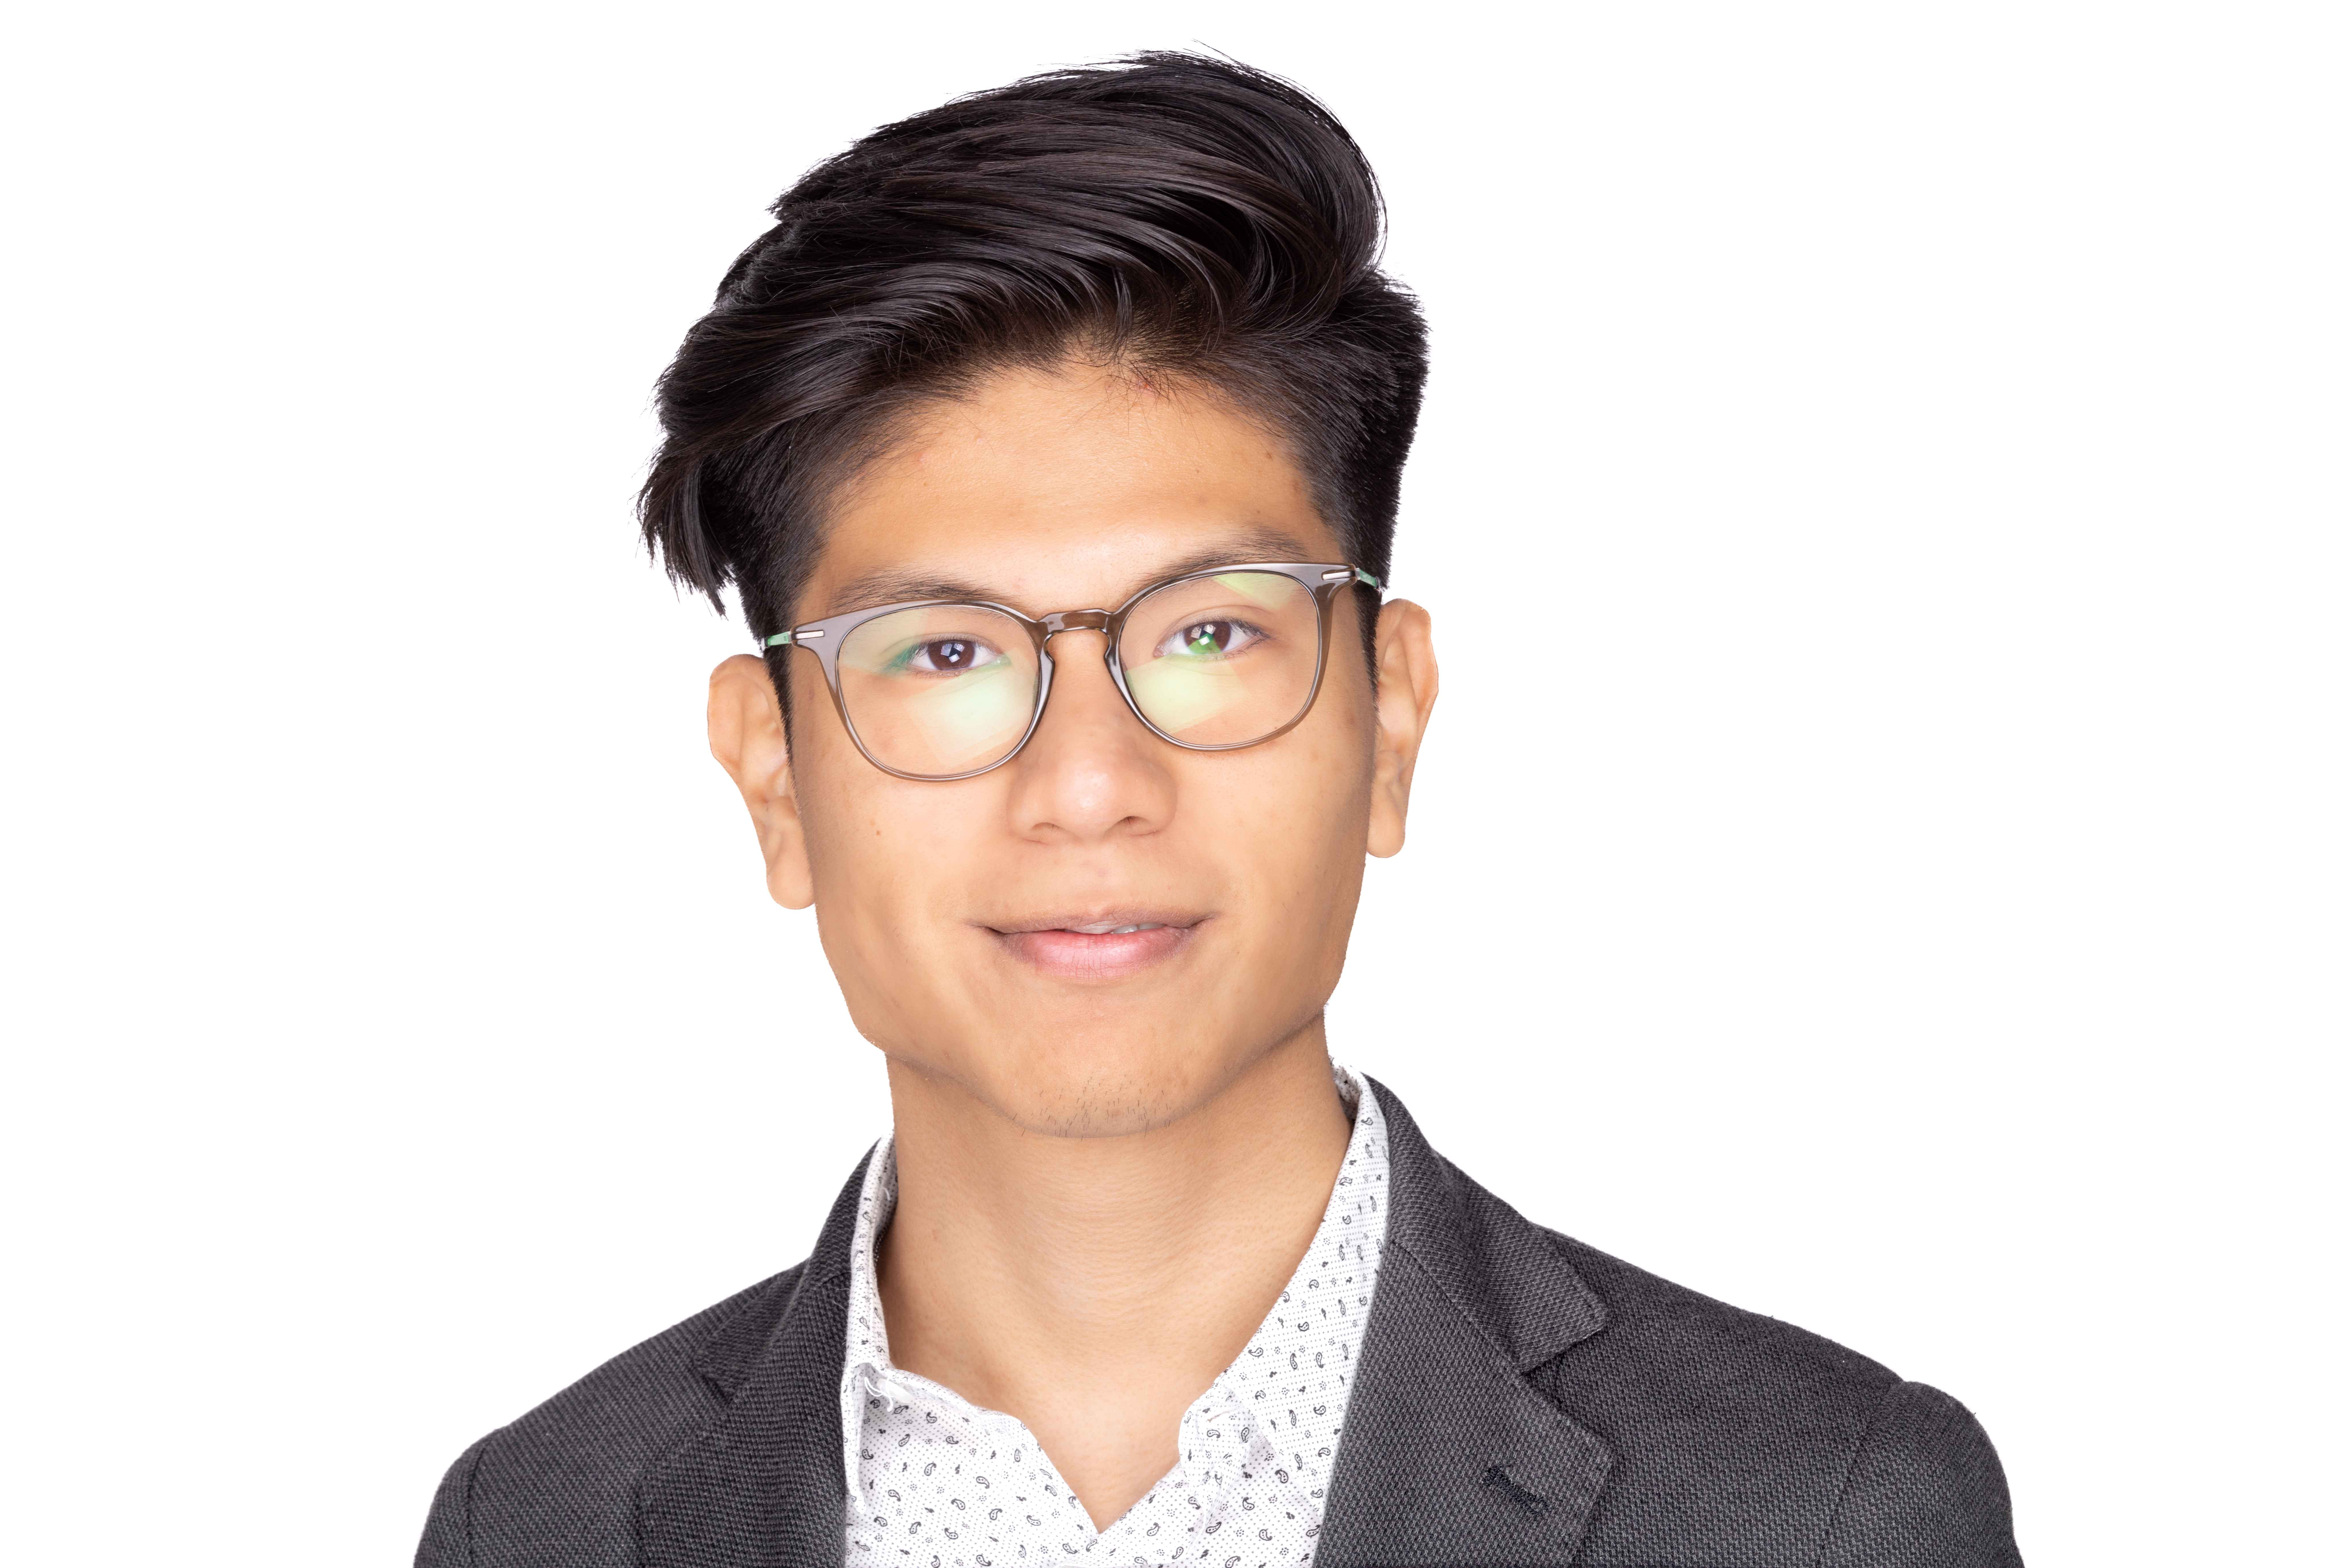
\includegraphics[width=\linewidth, trim={1cm 0cm 1cm 0cm}, clip]{profile-picture-compressed.jpg}};
        \end{tikzpicture}
    \end{minipage}

    \vspace{\sidespacing}

    % --- BIO -------------------------------------------------------------------------------
    \begin{rSection}{SUMMARY}
        \item A software engineer studying AI, dedicated to devops
        still using Vim \& tiling window managers in Linux
    \end{rSection}

    \vspace{\sidespacing}

    \begin{rSection}{STRONG SKILLS}
        \item Python, Django, Flask, FastAPI,
        \item Java, Spring Boot, Javascript, Vue
        \item Docker, Terraform, Networking
    \end{rSection}

    \vspace{\sidespacing}

    % --- CERTIFICATIONS --------------------------------------------------------------------
    \begin{rSection}{CERTIFICATIONS}
        \item \underline{CCNA} {CISCO, 2021}
        \item \underline{Comau} {Robots programming, 2020}
        \item \underline{ECDL} {AICA, 2019}
    \end{rSection}

    \vspace{\sidespacing}

    % --- LANGUAGES --------------------------------------------------------------
    \begin{rSection}{Languages}
        \vspace{0.2cm}
        \item \begin{tabular}{@{}ll@{}}
            English & Fluent + Certificates \\
            Italian & Native                \\
            Spanish & Native                \\
            French  & A2 Certificate        \\
            German  & Beginner              \\
        \end{tabular}
    \end{rSection}

    \vspace{\sidespacing}

    \begin{rSection}{Portfolio}
        \item[]
\includegraphics[width=\iconsize, trim={0cm 0.4cm 0cm 0cm}]{github-mark.png}
        \href{https://github.com/JekxDevil}{github.com/JekxDevil}

        \item[]
\includegraphics[width=\iconsize, trim={0cm 0.5cm 0cm 0cm}]{gitlab-icon.png}
        \href{https://gitlab.com/JekxDevil}{gitlab.com/JekxDevil}

        \item[]
\includegraphics[width=\iconsize, trim={0cm 0.12cm 0.03cm 0cm}]{website.png}
        \href{http://jefersonmm.com}{jefersonmm.com}
    \end{rSection}

    \vspace{\sidespacing}

    \begin{rSection}{Documents}
        \item[] EU Italian citizenship
        \item[] Swiss B permit work authorization
        \item[] Driving license B
    \end{rSection}

    % keyword injection for ATS
    \transparent{0}
    \tiny
    \begin{rSection}{Skills}
        \item[] git, shell scripting, uml, vagrant, solid, domain driven design,
        venv, pytest, gitflow, continuous integration, continuous deployment,
        gitops, junit, nginx, sonarqube, scrum, agile project management, containerization,
        orchestration,
        mongodb, sqlite, postgresql, mysql, % databases
        Vuejs, vuetify, nodejs, expressjs, web sockets, webRTC, material design, % frontend
        competitive programming, CTF, OOP, Java Swing, test driven development,
        functional programming, scheme, racket, lisp, d3.js, s3, OpenGL, valgrind, gdb, gcc
    \end{rSection}
    \normalsize
    \transparent{1}

    \vspace{1.8cm}
    Written in \href{https://github.com/JekxDevil/curriculum-vitae}{\LaTeX}.

\end{minipage}
\hspace{0.1cm}
\begin{minipage}[b][0.9\paperheight][t]{0.7\linewidth}

    \headline

    % --- OBJECTIVE -------------------------------------------------------------------------------
    \begin{rSection}{OBJECTIVE}
        \item Software engineer with 3+ years of experience in fullstack development specialized in backend,
        seeking Cloud and Network internship roles.
    \end{rSection}

    \begin{rSection}{Education}
        \vspace{0.2cm}
        % --- UNIVERSITY BACHELOR --------------------------------------------------------------------   
        %
\includegraphics[width=0.5cm, trim={0cm 5cm 0cm 0cm}]{usi-icon.png}
        
\includegraphics[width=0.7cm, trim={0cm 3cm 0cm 0cm}]{ethz-icon.png}
        {\bf Master in Computer Science}
        \hfill \href{https://ethz.ch/en.html}{ETH}, Switzerland
        \item \hspace{0.85cm}Major in Artificial Intelligence. %Minor in Data Management.
        \hfill {Sep 2024 - Present}
        \item Minor in Medical applications and Data Management.
        \vspace{\intraexpvspace}
        \vspace{\intraexpvspace}

        % --- UNIVERSITY BACHELOR --------------------------------------------------------------------   
        %
\includegraphics[width=0.5cm, trim={0cm 5cm 0cm 0cm}]{usi-icon.png}
        
\includegraphics[width=0.7cm, trim={0cm 10cm 0cm 0cm}]{usi-icon.png}
        {\bf Bachelor in Computer Science}
        \hfill \href{https://www.usi.ch/en}{USI}, Switzerland
        \item \hspace{0.85cm}Scholarship. Degree in English. GPA 5.59/6.
        \hfill {Sep 2021 - Jun 2024}
        \item Specialization in computational science: \textbf{Matlab}, graphs, numerical optimization.
        \vspace{\intraexpvspace}
        \vspace{\intraexpvspace}

        % --- School -------------------------------------------------------------------------
        
\includegraphics[width=0.7cm, trim={0cm 2.2cm 0cm 0cm}]{iisve-icon.png}
        {\bf High School Diploma in Computer Science}
        \hfill \href{https://www.istitutovolterraelia.it/}{IIS Volterra Elia}, Italy
        \item \hspace{0.85cm}Graduated with Honors.
        \hfill {Sep 2016 - Jun 2021}
        \item Specialization in .Net framework: \textbf{C\#}, Windows Forms, MS SQL Server, ASPX
    \end{rSection}
    % --- WORK EXPERIENCE -------------------------------------------------------------------   
    \begin{rSection}{EXPERIENCE}
        \vspace{0.2cm}

        %--- TA --------------------------------------------------------------------------------
        
\includegraphics[width=0.7cm, trim={0cm 10cm 0cm 0cm}]{usi-icon.png}
        \hspace*{0cm}\textbf{Teaching Assistant} \hfill Feb - Jun 2024\\
        \hspace*{0.85cm}\href{https://www.usi.ch/}{USI} Università della Svizzera italiana
        \hfill \textit{Lugano, Switzerland}
        \begin{itemize}
            \item \href{https://search.usi.ch/it/corsi/35268192/software-atelier-4-software-engineering-project}{Software Engineering}:
                  requirements engineering, \textbf{Spring Boot}, \textbf{Vue}, \textbf{devops}.
                  % course by Dr. A. Mocci

            \item \href{https://search.usi.ch/it/corsi/35268184/data-management}{Data Management}:
                  relational databases, transaction query processing, \textbf{Spark}.
                  % course by Prof. P. T. Eugster
        \end{itemize}
        \vspace{\intraexpvspace}
        \vspace{\intraexpvspace}

        %--- Claranet ----------------------------------------------------------------------------
        
\includegraphics[width=0.7cm, trim={0cm 15cm 0cm 0cm}]{claranet-logo.png}
        \textbf{Cloud Developer} \hfill Sep - Dec 2023\\
        \hspace*{0.85cm}\href{https://www.claranet.com/}{Claranet} - Cloud Service Provider
        \hfill \textit{Lugano, Switzerland}
        \begin{itemize}
            \item Provisioning infrastructure with \textbf{Terraform} and \textbf{Cloudformation}
                  IaC tools.

            \item Designed cloud assessment challenges with boto3 and \textbf{AWS} services.
                  % with real time evaluation in SOAR assessment platform.
                  % Assigning time constrained challenges with grading based 
                  % on solution functionality and cloud conventions compliancy.
        \end{itemize}
        \vspace{\intraexpvspace}
        \vspace{\intraexpvspace}

        %--- UROP --------------------------------------------------------------------------------
        
\includegraphics[width=0.7cm, trim={0cm 10cm 0cm 0cm}]{si-icon.jpg}
        \hspace*{0cm}\textbf{Undergraduate Student Researcher} \hfill Jul - Aug 2022\\
        \hspace*{0.85cm}\href{https://www.si.usi.ch/}{USI Software Institute},
        \href{https://luce.si.usi.ch/team/}{LuCE} research lab
        \hfill \textit{Lugano, Switzerland}
        \begin{itemize}
            \item Created backend with \textbf{FastAPI} to convert \textbf{Python} programs' AST
                  into an expression-based notional machine retaining equivalent structure.
                  % Part of \textit{Expression tutor} webapp 
                  % for assessment of structure, typing, and evaluation of expressions.
                  % with usage of design patterns 
                  % for parsing and exploring source code graph structures.
        \end{itemize}
        \vspace{\intraexpvspace}
        \vspace{\intraexpvspace}

        %--- IDEA -------------------------------------------------------------------------------
        
\includegraphics[width=0.75cm, trim={0cm 1.5cm 0cm 0cm}]{idea-icon.png}
        \textbf{Software Developer} \hfill Feb, Jun - Aug 2020; Jul 2021\\
        \hspace*{0.85cm}\href{https://idea-on-line.it/}{Idea Soc Coop} - Industrial Automation
        \hfill \textit{Ancona, Italy}
        \begin{itemize}
            \item Blood bag logger:
                  developed embedded web app for data visualization in \textbf{Flask}.

            \item Environmental sensor:
                  sketched micropython firmware with \textbf{AWS Alexa} skill.
        \end{itemize}
        \vspace{\intraexpvspace}
        \vspace{\intraexpvspace}

        %-- BitService --------------------------------------------------------------------------
        
\includegraphics[width=0.75cm, trim={0cm 1.5cm 0cm 0cm}]{bitservice-icon.png}
        \textbf{ICT technician} \hfill May 2019 \\
        \hspace*{0.85cm}BitService di Santoni Angelo - IT Consulting
        \hfill \textit{Ancona, Italy}
        %\begin{itemize}
        %    \item Hardware and OS maintenance, GDPR compliance, Moodle e-learning.
        %\end{itemize}
    \end{rSection}

    %--- PROJECTS SECTION -------------------------------------------------------------------
    \begin{rSection}{PROJECTS}
        \item \textbf{\href{https://pufferfish.sa4.usi.ch/login}
            {
                JourneyTales
                
\includegraphics[width=0.15cm, trim={10cm -10cm 0cm 0cm}]{ext-link-icon.png}
            }}
        {Leader, 12 developers team.
            Built \textbf{social media} to share travel experiences,
            with friendship mechanisms and realtime notifications.
            \textbf{Responsive} web application with \textbf{OAuth2} and $\boldsymbol{> 99\%}$ \textbf{test} coverage.
            \href{https://gitlab.com/usi-si-oss/teaching/projects-showcase/sa4/team-4-pufferfish}{GitLab.}
        }

        \vspace{\intraexpvspace}
        \item \textbf{\href{https://handshakeapp.ch}{
                Handshake
                
\includegraphics[width=0.15cm, trim={10cm -10cm 0cm 0cm}]{ext-link-icon.png}
            }}
        {Built an \textbf{instant messaging} web application with video calls, group chats and friends
            using MEVN stack deployed on AWS.
            During \textbf{presentation $\boldsymbol{\approx1000}$ messages from $\boldsymbol{+ 80}$ users}.
            Team of 5 developers.
            \href{https://github.com/ogs-at-usi/handshake}{GitHub}.
        }
    \end{rSection}
    %--- LEADERSHIP -------------------------------------------------------------------------
    \begin{rSection}{Leadership \& Achievements}
        \vspace{0.2cm}
        \begin{itemize}[leftmargin=*]
            \itemsep 0.2em
            \item \textbf{Swiss Scholarship} awarded at USI from
                  \href{https://www.olimpiadi-informatica.it/index.php/selezione-territoriale-20.html}{Italian Informatics Olympiad 2020}.
                  %FFL, scoring a remarkable ranking.

            \item \href{https://icpc.global/ICPCID/ZOI3HF9XDUH8}{ICPC SWERC 2022}
                  competed as USInchronous team representing USI.

            \item Included in Italian \href{https://www.indire.it/eccellenze/}{National Register of Excellence} 2020/2021.

            \item \href{https://www.makerslab.it/olimpiadi-robotiche-ancona-2019/}{1st team}
                  classified in \textbf{Robotics} Olympiad 2019 regional phase in Italy. % Contest Marche region, Ancona.

            \item \href{https://cyberchallenge.it/}{CyberChallenge} 2019 \textbf{youngest} student
                  in \textit{Marche}, Italy. Cybersecurity course. % Cybersecurity National Lab.

            \item \textbf{Faculty Representantive} of \textbf{Informatics} in the student council at USI.

            \item \href{https://hackzurich.com/}{HackZurich},
                  \href{https://www.junction2023.com/}{Junction}
                  hackathon participations in \textbf{Zurich} and \textbf{Helsinki}.
                  % $2022$ \& $2023$; 2023 with leader role 
        \end{itemize}
    \end{rSection}

\end{minipage}
\end{document}

%!!!!!!!!!!!!!!!!!!!!!!!!!!!!!!!!!!!!!!!!!!%%%%%%%%%%%%%%%%%%%%%%%%%%%%%%%%%%%%%%%%%%%%%%%%%%%%%%%%%%%%%%%%%%%
%--- OBJECTIVE --------------------------------------------------------------------------
%\begin{rSection}{OBJECTIVE}
%{Software Engineer with 2+ years of experience in XXX, seeking full-time XXX roles.}
%\end{rSection}
%%%%%%%%%%%%%%%%%%%%%%%%%%%%%%%%%%%%%%%%%%%%%%%%%%%%%%%%%%%%%%%%%%%%%%%%%%%%%%%%%%%%%%%%
%%Technical Skills & MongoDB, Vuejs, Express, Nodejs, Windows Forms, Visual Studio, 
FastAPI, Java, Java Swing, Java Spring Boot, Docker D \\

ICPC SWERC 2022 participation: Participated in the International Collegiate Programming Contest,
Southwestern Europe Regional. Competed as USInchronous team representing USI.

EXTRACURRICULAR:
Sea lifeguard license. Società Nazionale di Salvamento, Issued Jul 2019. Credential ID 631357.
Computer assembling, hardware and custom PC builds.
Participating in CyberSecurity CTFs competitions.
OpenBSD enjoyer, GNU/Linux as daily drive.
Vim and tiling window managers enthusiast (i3, dwm), suckless software connoisseur
Theater actor at Iride Theater Company.

TODO: add to portfolio

PROJECTS:
Risk-Kellogs: https://github.com/micheledallerive/Risk-Kelloggs
Pair Programming, Test Driven Development. Modeled Risiko board game, object oriented paradigm
Java Swing, design patterns, event driven, SOLID, OOP paradigm

Pacman-Racket: https://github.com/JekxDevil/pacman-racket
Leading a team of 4 developers. Remake of Pacman classic game in functional paradigm.
Scheme, immutability, vim, functional paradigm,

Merendero: Built a CRUD app for secondary school connected to MS SQL server database
using windows forms for GUI implementation and C# with .Net Framework.

UNIVERSITY:
Programming Fundamentals:
- Functional in Racket, a LISP dialect
- Imperative, Procedural, OOP in Java
- Concurrency in Java
Software Ateliers:
- Fundamentals of Informatics
- UI/UX Design
- Web Development with MEVN stack
- Software Engineering + Course Project using Java Spring Boot
Mathematical oriented courses:
- Calculus
- Linear Algebra
- Discrete Structures
- Probability & Statistics
- Computational Science Theory
Algorithms & Data Structures in Python3
Computer Architecture, Operating Systems in C
Systems Programming in C++
Automata & Formal Languages
Computer Networking
Electives:
Programming Challenges in Competitive Programming style
Programming Fundamentals: - Functional in Racket, a LISP dialect - Imperative, Procedural, OOP in Java - Concurrency in Java
Software Ateliers: - Fundamentals of Informatics - UI/UX Design - Web Development with MEVN stack - Software Engineering + Course Project using Java Spring Boot
Mathematical oriented courses: - Calculus - Linear Algebra - Discrete Structures - Probability & Statistics - Computational Science Theory
Algorithms & Data Structures in Python3 Computer Architecture,
Operating Systems in C Systems Programming in C++
Automata & Formal Languages
Computer Networking
Electives: Programming Challenges in Competitive Programming style

MICROSOFT: .Net, C#, Windows forms, SQL server, ASPX

HIGH SCHOOL:
HTML, CSS, javascript, C++, Java, PHP, Joomla
Developed full stack web apps and resource management desktop applications with database connection.
CRUD Merendero, Full stack web development and programming language paradigms,
Networking: ISO/OSI stack, CISCO networking, threads, sockets
Telecommunications: arduino embedded prototyping, analogic/digital electronic components
Mathematics, Sciences: Physics, Chemistry, Biology, Geography

CERTIFICATIONS:
CCNA, CISCO Routing and Switching, 2021.
Cisco Networking Academy Issued May 2021. Credential ID 1016658774.

Comau Use and Programming for C5G family of robots, 2020
Issued Nov 2020. Credential ID WmN8DebufQ.

CyberChallenge Student Issued Jul 2019.

ICDL Full Standard, AICA. Issued May 2019. Credential ID IT2159274.

COMPUTATIONAL SCIENCE:
Matlab, graph partitioning & clustering, conjugate gradient, page rank,
least squares, data fitting, Analysis
optimization methods, numerical computing, statistics,
linear algebra, discrete maths, calculus

FROTEND:
UI/UX design in Figma, Software Engineering: fullstack web development.
Balsamiq wireframes prototyping.

DATABASES:
MySQL, relational databases
mongodb, document based

EXTRA:
Attended the ACM ICSA International Symposium on Computer Architecture 2022
workshops and office hours
Sea lifeguard. Casual guitarist. Actor.
Vim and tiling window managers enthusiast.
OpenBSD enjoyer, GNU \text{+} Linux as daily drive.
CTFs cybersecurity participant.
Suckless software connoisseur.
Electives: Programming Challenges in Competitive Programming style @ USI

EMBEDDED:


SOFT SKILLS:
flexibility, public speaking, resilient,  pressure performer, attention to detail


ALGORITHMS:
algorithms & data structures, experimetation & evaluation, automata & formal languages regex

LOW LEVEL GRAPHICS
Computer Graphics, Systems Programming, Operating Systems, Computer Architecture
raytracing, OpenGL, WebGL, gcc, gdb, C, C++, valgrind, makefile, x86 assembly, multithreading, vagrant, concurrency, BSD kernel

NETWORKING:
Networking, Information Retrieval, data management, web design
wireshark, web crawling, Search engine, Terrier IR, Scrapy, python, subnetting,

SOFT SKILLS TAs:
project management, Agile development, design patterns

CLARANET KEYWORDS: lambda, API Gateway, S3, IAM, serverless, Cloud9, IaC, devops


BITSERVICE DESCRIPTION: Improved websites with wordpress. Profiling GDPR compliance. Created
moodle e-learning content for it. EU regulations. Building, setup and maintenance
of computer hardware, OS and software
KEYWORDS: Wordpress, EU GDPR, Moodle, computer building/assembling

IDEA Projects: BOSET blood bag logger, DONET environmental sensors device
docking station RaspberryPI, porting company's SCADA to newer version of Ignition with Python3
KEYWORDS: d3.js, aws iot, sqlite, linux, nfc, esp32